\documentclass[letterpaper,12pt]{article}
\usepackage[utf8]{inputenc}
\pagestyle{empty}
\usepackage{amsmath,amssymb}
%\usepackage[activeacute,spanish]{babel}
\usepackage{ucs}
%\usepackage[applemac]{inputenc}
%\usepackage[T1]{fontenc} tipo de letra
\usepackage[scaled]{berasans}
\usepackage{amssymb}
\usepackage{amsmath,latexsym,amsthm,mathrsfs}
\usepackage{setspace}
\usepackage{psfrag}
\usepackage{graphicx}
\usepackage{enumerate}
\usepackage{float}
\usepackage{multirow,array}

\usepackage{caption}
\usepackage{subcaption}


\usepackage{tikz}
\usepackage{tkz-graph}
\usetikzlibrary{arrows,%
                petri,%
                topaths}%
%\usepackage{tkz-berge}
%\usepackage[position=top]{subfig}

%\usepackage[spanish]{babel}
\newcommand{\R}{\mathbb{R}}
\newcommand{\F}{\mathcal{F}}
\newcommand{\T}{\mathcal{T}}
\newcommand{\A}{\mathcal{A}}
\newcommand{\B}{\mathcal{B}}
\newcommand{\PP}{\mathbb{P}}
\newcommand{\EE}{\mathbb{E}}
\newcommand{\VV}{\mathbb{V}ar}
\newcommand{\naturales}{n\in\mathbb{N}}
\newcommand{\N}{\mathbb{N}}
\newcommand{\NN}{\mathbb{N}}
\newcommand{\p}{\partial}
\newcommand{\ssi}{\Leftrightarrow}
\newcommand{\imp}{\Rightarrow}
\newcommand{\Ssi}{\Longleftrightarrow}
\newcommand{\Imp}{\Longrightarrow}
\newcommand{\ind}{\mathds{1}}
%\renewcommand*\familydefault{\sfdefault}
%\usepackage[charter]{mathdesign}
%\usepackage{dsfont} 
\usepackage{multicol}
\usepackage{anysize}
\newtheorem{definicion}{Definición}
\newtheorem{proposicion}{Proposición}
\newtheorem{lema}{Lema}
\newtheorem{teorema}{Teorema}
\newtheorem{hint}{Hint}


\usepackage[left=1.5cm,top=2cm,right=1.5cm, bottom=1.5cm]{geometry}

\usepackage{fancyhdr}


\newtheorem{Def}{Definición}

\begin{document}




\begin{center}
	 \bf{Control 2: IN7K1 Teoría de Juegos, 2016}
\end{center}

%\begin{flushleft}


\begin{enumerate}[\bf P1.]

\item
Dos bienes indistinguibles serán rematados entre $n$ agentes cuya valoración por el bien sigue una distribución $F$ y son independientes. Cada agente desea obtener solo uno de los bienes, es decir, nunca se asigna dos veces al mismo comprador. En este contexto:
 \begin{itemize} 
     \item[a)] Describa la asignación y los pagos de un mecanismo VCG.
     \item[b)] Pruebe que sigue siendo válido el teorema de equivalencia de ingresos.
     \item[c)] Asumiendo $F$ regular, encuentre la regla de asignación para un remate de Myerson.
     \item[d)] Para un mecanismo de posted price, formule una expresión para encontrar el mejor precio fijo (el precio que maximiza la utilidad del martillero cuando su estrategia es cobrar el mismo precio a todos los cliente).
     \item[e)] Calcule el ingreso del martillero en las partes \textbf{a)}, \textbf{c)} y \textbf{d)} cuando $n=3$ y $F\sim U[0,1]$.
\end{itemize}
\item En el grafo de la Figura 1 están representadas las preferencias de tres alumnos $a_1$, $a_2$ y $a_3$ sobre tres colegios $c_1$, $c_2$ y $c_3$ con capacidad unitaria (y viceversa).
\begin{itemize}
    \item[a)] Encuentre el resultado de aplicar DA y eliminación.
    \item[b)] Considere la situación de la Figura 2, donde un matching estable sobre un conjunto de estudiantes y colegios ha asignado $\{a_1,c_2\}$ y $\{a_2,c_1\}$. Pruebe que $a_2\succeq_{c_1} a_1$ y $a_1\succeq_{c_2} a_2$. Demuestre además que todo matching estable $\mu$ cumple que $\mu(a_1)=c_2$ y $\mu(a_2)=c_1$.
    \item[c)] Encuentre el resultado de aplicar TTC sobre el grafo de la Figura 1.
    \item[d)] Considere el problema de matching unisex, donde cada uno tiene preferencias sobre resto, y el número de agentes es par. Defina la noción de matching estable para este caso y determine los matchings estables cuando las preferencias están dadas por la Tabla 1. >Qu\'e puede concluir?

 \begin{figure}[H]
 \centering
 \begin{minipage}{.3\textwidth}
 \centering
 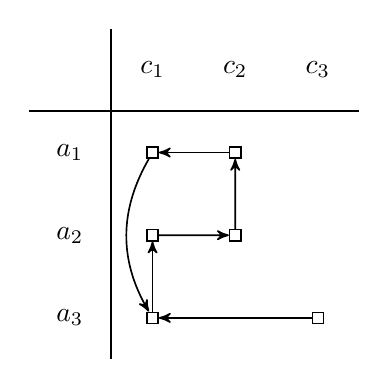
\begin{tikzpicture}[scale=2.1,>=stealth', semithick, auto]
    \tikzstyle{lab}=[ineer sep=1pt]
    \tikzstyle{agent}=[circle, draw=none, minimum width=2pt, inner sep=2pt]
    \tikzstyle{vert}=[rectangle, draw, minimum width=2pt, inner sep=2pt]
    
    \node[agent] (a1) at (0,-1/2) {$a_1$};
    \node[agent] (a2) at (0,-1) {$a_2$};
    \node[agent] (a3) at (0,-1.5) {$a_3$};
    \node[agent] (c1) at (1/2,0) {$c_1$};
    \node[agent] (c2) at (2/2,0) {$c_2$};
    \node[agent] (c3) at (3/2,0) {$c_3$};
    
    \node[vert] (11) at (1/2,-1/2) {};
    \node[vert] (12) at (1,-1/2) {};
    \node[vert] (21) at (1/2,-1) {};
    \node[vert] (22) at (1,-1) {};
    \node[vert] (31) at (1/2,-3/2) {};
    \node[vert] (33) at (3/2,-3/2) {};
    
    \draw[->, bend right=30, looseness=1] (11) edge (31);
    \draw[->] (31) edge (21);
    \draw[->] (33) edge (31);
    \draw[->] (12) edge (11);
    \draw[->] (22) edge (12);
    \draw[->] (21) edge (22);
    
    \draw[-] (-1/4,-1/4) edge (7/4,-1/4);
    \draw[-] (1/4,1/4) edge (1/4,-7/4);
    
\end{tikzpicture}
\captionof*{figure}{Figura 1}
\label{fig:f1}
  
\end{minipage}%
\begin{minipage}{.3\textwidth}
 \centering
 \begin{tikzpicture}[scale=2.1,>=stealth', semithick, auto]
    \tikzstyle{lab}=[ineer sep=1pt]
    \tikzstyle{agent}=[circle, draw=none, minimum width=2pt, inner sep=2pt]
    \tikzstyle{vert}=[rectangle, draw, minimum width=2pt, inner sep=2pt]
    \tikzstyle{vertn}=[rectangle, draw, minimum width=2pt, inner sep=2pt, fill=black]
    
    \node[agent] (a1) at (0,-1/2) {$a_1$};
    \node[agent] (a2) at (0,-1) {$a_2$};
    \node[agent] (a3) at (0,-1.5) {$\vdots$};
    \node[agent] (c1) at (1/2,0) {$c_1$};
    \node[agent] (c2) at (2/2,0) {$c_2$};
    \node[agent] (c3) at (3/2,0) {$\cdots$};
    
    \node[vert] (11) at (1/2,-1/2) {};
    \node[vertn] (21) at (1/2,-1) {};
    \node[vert] (22) at (1,-1) {};
    \node[vertn] (12) at (1,-1/2) {};    

    \draw[->] (12) edge (11);
    \draw[->] (21) edge (22);
    
    \draw[-] (-1/4,-1/4) edge (7/4,-1/4);
    \draw[-] (1/4,1/4) edge (1/4,-7/4);
    
\end{tikzpicture}
\captionof*{figure}{Figura 2}
\label{fig:f2}
  
\end{minipage}%
\begin{minipage}{.3\textwidth}
\centering
\begin{tabular}{|c|c|}
    \hline
    $a$ & $b \succeq c \succeq d$ \\
    $b$ & $c \succeq a \succeq d$ \\
    $c$ & $a \succeq b \succeq d$ \\
    $d$ & $a \succeq b \succeq c$ \\
    \hline
\end{tabular}
\captionof*{figure}{Tabla 1}
\label{tab:t1}
     
  
\end{minipage}%


\end{figure}
 
\end{itemize}



\item En este problema queremos comparar las ganancias esperadas en un remate óptimo con $n$ jugadores, versus un remate a segundo precio (VCG) con $n+1$ jugadores. Para el problema suponga que las distribuciones de las valoraciones de cada jugador son regulares. 
\begin{itemize}
\item[a)] Considere un remate sobre $n$ jugadores donde siempre se asigne el objeto. Recordando el problema de Myerson (En particular la equivalencia entre dos funciones objetivo) argumente cual es el remate óptimo con la propiedad de siempre asignar el objeto.

\item[b)] Diseñe un mecanismo con $n+1$ jugadores donde el objeto siempre sea asignado y la ganancia esperada sea la misma que la del remate óptimo con $n$ jugadores.

\item[c)] Usando la regularidad de las distribuciones y la primera parte, vea como puede comparar el remate anterior con el remate a segundo precio entre $n+1$ jugadores. ¿Que puede concluir?
\end{itemize}


\end{enumerate}
%\end{flushleft}
\end{document}
